% SC4022 --- Chapter 8: Applications (Social, Biological, Technological) (0->100 ground-up)
\chapter{Applications: Social, Biological \& Technological Networks}
\label{ch:applications}
\sloppy

\begin{quote}
\emph{``The same math in different clothes.''} --- Friendship, protein binding, and router links obey the same network laws yet reveal domain-specific stories. Seeing one lens through three domains cements the whole picture.
\end{quote}

\noindent\fbox{\parbox{\dimexpr\linewidth-2\fboxsep-2\fboxrule}{%
\textbf{From zero: we build here, no domain background needed.} We assume only Ch.~1--7 (graph, centrality, community, random/scale-free, spreading, robustness). Each domain is introduced from scratch, then analysed with tools from earlier chapters.}}
\vspace{0.4em}

\section*{Learning Outcomes}
After this chapter you will be able to:
\begin{enumerate}[label=(L\arabic*)]
    \item map and interpret social networks: homophily, triadic closure, and influence;
    \item analyse biological networks: PPI hubs as essential proteins, metabolic and neural motifs;
    \item dissect technological networks: WWW bow-tie, Internet AS-graph, power-grid fragility;
    \item synthesise universal vs domain-specific patterns across the three domains;
    \item conduct a capstone mini-project: collect, measure, visualise, and report on a real dataset.
\end{enumerate}

% ============================================================
\section{Social Networks}
\label{sec:social}
\paragraph{Intuition.} People befriend those nearby and those like themselves (\emph{homophily}), and friends of friends tend to become friends (\emph{triadic closure}---closing a triangle). These micro-mechanisms create high clustering and communities by age, interest, or workplace. A collaboration network (authors linked if they co-authored) is bipartite authors--papers projected onto authors; its communities are research fields.

Standard traits: heavy-tailed degrees (a few super-connectors), high $C$, positive degree assortativity (hubs connect to hubs), and community structure. Centrality here predicts influence; spreading models capture rumour or adoption (Ch.~6 threshold models fit better than simple SIR because social adoption often needs reinforcement).

\begin{figure}[h]\centering
\begin{tikzpicture}[scale=0.82,every node/.style={font=\scriptsize}]
\begin{scope}
\node[font=\footnotesize\bfseries] at (1.6,2.85) {Social};
\node[circle,draw,thick,fill=blue!16,minimum size=0.68cm] (s1) at (0.4,1.8) {A};
\node[circle,draw,thick,fill=blue!16,minimum size=0.68cm] (s2) at (1.6,2.2) {B};
\node[circle,draw,thick,fill=blue!16,minimum size=0.68cm] (s3) at (2.8,1.8) {C};
\node[circle,draw,thick,fill=green!14,minimum size=0.68cm] (s4) at (0.6,0.6) {D};
\node[circle,draw,thick,fill=green!14,minimum size=0.68cm] (s5) at (2.2,0.6) {E};
\draw[thick] (s1)--(s2)--(s3); \draw[thick] (s4)--(s5); \draw[thick] (s1)--(s4); \draw[thick] (s3)--(s5);
\draw[thick,red!70!black,dashed,line width=0.9pt] (s2)--(s4);
\node[font=\tiny,fill=red!10,rounded corners=2pt,inner sep=2pt] at (1.6,0.0) {dashed = triadic closure};
\end{scope}
\begin{scope}[xshift=4.6cm]
\node[font=\footnotesize\bfseries] at (1.6,2.85) {Biological (PPI)};
\node[circle,draw,thick,fill=red!16,minimum size=0.70cm] (p1) at (1.6,1.6) {Hub};
\foreach \a in {20,70,120,170,220,270,320} {\node[circle,fill=orange!12,draw,minimum size=0.44cm] at ($(p1)+(\a:1.0)$) {}; \draw[thick,orange!60!black] (p1)--($(p1)+(\a:1.0)$);}
\node[font=\tiny,fill=red!10,rounded corners=2pt,inner sep=2pt] at (1.6,0.0) {hub = essential protein};
\end{scope}
\begin{scope}[xshift=9.0cm]
\node[font=\footnotesize\bfseries] at (1.4,2.85) {Technological};
\node[circle,draw,thick,fill=violet!14,minimum size=0.60cm] (t1) at (0.5,1.7) {R1};
\node[circle,draw,thick,fill=violet!14,minimum size=0.60cm] (t2) at (2.0,1.9) {R2};
\node[circle,draw,thick,fill=violet!14,minimum size=0.60cm] (t3) at (1.4,0.7) {R3};
\draw[thick,violet!60!black] (t1)--(t2)--(t3)--(t1);
\draw[thick,violet!60!black] (t1)--(t3);
\node[font=\tiny,fill=violet!10,rounded corners=2pt,inner sep=2pt] at (1.4,0.0) {routers / power buses};
\end{scope}
\node[font=\tiny,draw=gray!40,fill=yellow!8,rounded corners=2pt,inner sep=3pt] at (4.8,-0.55) {\textcolor{blue!60!black}{$\blacksquare$ social} \quad \textcolor{orange!60!black}{$\blacksquare$ PPI hub} \quad \textcolor{violet!60!black}{$\blacksquare$ tech} \quad triadic closure vs hub essentiality};
\end{tikzpicture}
\caption{Three domains, same language. Social: communities and triadic closure (red dashed is a triangle closing). Biological: a few hub proteins bind many partners---hubs are essential. Technological: router/power grids are engineered, more regular but still with hubs.}
\label{fig:three-domains}
\end{figure}

% ============================================================
\section{Biological Networks}
\label{sec:bio}
\paragraph{Intuition.} In a protein--protein interaction (PPI) network, nodes are proteins, edges are bindings. Removing a hub protein often kills the cell (lethality--centrality rule), while removing a leaf does not---a direct analogue of Ch.~7 targeted attack. Metabolic networks are bipartite (metabolites + reactions) and hierarchical; neural networks (e.g.\ \emph{C.~elegans} 302 neurons) are small-world with modules for function and a rich club of hub neurons interconnecting modules.

Traits that differ from social: PPI is disassortative (hubs avoid hubs, to separate functions), clustering is moderate, and motifs matter---feed-forward loops and bifans appear far more than in random nulls (use configuration model with same degrees as null, as in Ch.~4).

\begin{figure}[h]\centering
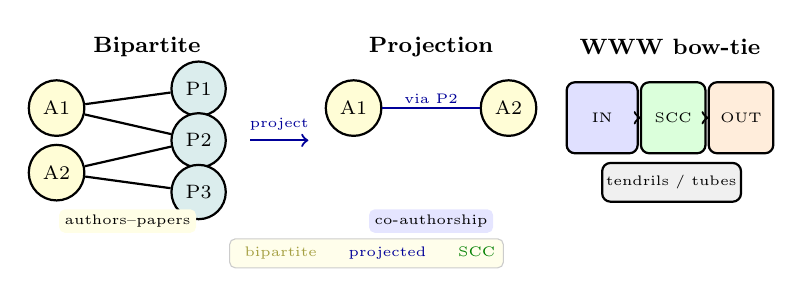
\begin{tikzpicture}[scale=0.82,every node/.style={font=\scriptsize}]
% bipartite projection
\node[font=\footnotesize\bfseries] at (1.4,2.55) {Bipartite};
\node[circle,draw,thick,fill=yellow!16,minimum size=0.60cm] (u1) at (0,1.6) {A1};
\node[circle,draw,thick,fill=yellow!16,minimum size=0.60cm] (u2) at (0,0.6) {A2};
\node[circle,draw,thick,fill=teal!14,minimum size=0.60cm] (v1) at (2.2,1.9) {P1};
\node[circle,draw,thick,fill=teal!14,minimum size=0.60cm] (v2) at (2.2,1.1) {P2};
\node[circle,draw,thick,fill=teal!14,minimum size=0.60cm] (v3) at (2.2,0.3) {P3};
\draw[thick] (u1)--(v1); \draw[thick] (u1)--(v2); \draw[thick] (u2)--(v2); \draw[thick] (u2)--(v3);
\node[font=\tiny,fill=yellow!10,rounded corners=2pt,inner sep=2pt] at (1.1,-0.15) {authors--papers};
\draw[->,thick,blue!60!black] (3.0,1.1)--(3.9,1.1) node[midway,above,font=\tiny] {project};
% projection
\begin{scope}[xshift=4.6cm]
\node[font=\footnotesize\bfseries] at (1.2,2.55) {Projection};
\node[circle,draw,thick,fill=yellow!16,minimum size=0.64cm] (w1) at (0,1.6) {A1};
\node[circle,draw,thick,fill=yellow!16,minimum size=0.64cm] (w2) at (2.4,1.6) {A2};
\draw[thick,blue!60!black,line width=1.0pt] (w1)--(w2) node[midway,above,font=\tiny,fill=white,inner sep=1pt] {via P2};
\node[font=\tiny,fill=blue!10,rounded corners=2pt,inner sep=2pt] at (1.2,-0.15) {co-authorship};
\end{scope}
% bow-tie WWW
\begin{scope}[xshift=8.0cm]
\node[font=\footnotesize\bfseries] at (1.5,2.55) {WWW bow-tie};
\draw[thick,fill=blue!12,rounded corners=3pt] (-0.1,0.9) rectangle (1.0,2.0); \node[font=\tiny] at (0.45,1.45) {IN};
\draw[thick,fill=green!14,rounded corners=3pt] (1.05,0.9) rectangle (2.05,2.0); \node[font=\tiny] at (1.55,1.45) {SCC};
\draw[thick,fill=orange!14,rounded corners=3pt] (2.10,0.9) rectangle (3.10,2.0); \node[font=\tiny] at (2.60,1.45) {OUT};
\draw[thick,fill=gray!12,rounded corners=3pt] (0.45,0.15) rectangle (2.60,0.75); \node[font=\tiny] at (1.52,0.45) {tendrils / tubes};
\draw[->,thick] (1.0,1.45)--(1.05,1.45); \draw[->,thick] (2.05,1.45)--(2.10,1.45);
\end{scope}
\node[font=\tiny,draw=gray!40,fill=yellow!8,rounded corners=2pt,inner sep=3pt] at (4.8,-0.65) {\textcolor{yellow!60!black}{$\blacksquare$ bipartite} \quad \textcolor{blue!60!black}{$\blacksquare$ projected} \quad \textcolor{green!50!black}{$\blacksquare$ SCC}};
\end{tikzpicture}
\caption{Left: bipartite author--paper network projected onto co-authorship (shared paper = edge). Right: the WWW bow-tie (Broder et~al.)---IN can reach SCC, SCC can reach OUT, tendrils hang off. Each domain reuses the same Ch.~1--7 machinery.}
\label{fig:bipartite-bowtie}
\end{figure}

% ============================================================
\section{Technological Networks}
\label{sec:tech}
\paragraph{Intuition.} The Web graph is directed (hyperlinks), heavy-tailed in-degree, and bow-tie shaped (Fig.~\ref{fig:bipartite-bowtie} right): a strongly connected core (SCC) where every page reaches every other, an IN that can reach the core, an OUT reachable from the core, plus tendrils. PageRank (Ch.~2) was invented for this graph. The Internet's autonomous-system (AS) graph is scale-free and disassortative; power grids are more lattice-like, with exponential degree tails---engineered for redundancy, yet vulnerable to cascades (Ch.~7).

% ============================================================
\section{Universal vs Specific and Capstone}
\label{sec:capstone}
Universals across domains: heavy-tailed degrees (often, but test via Ch.~5 Clauset), small-world (high $C$, short $L$), communities (Ch.~3), and hub-driven spreading/robustness (Ch.~6--7). Specifics: social is assortative and clustered; bio is disassortative and motif-rich; tech is engineered---Web is directed and bow-tie, power grid is not scale-free. Recognising both prevents over-generalising ``everything is scale-free.''

\paragraph{Capstone workflow.} Pick a dataset (Zachary karate, Les Mis\'erables co-appearance, \emph{C.~elegans} neural, or SNAP power grid). Then: collect/clean $\to$ measure ($n,m,\langle k\rangle,P(k),C,L$) $\to$ null test (ER / configuration) $\to$ centrality + community $\to$ simulate SIR and robustness $\to$ visualise $\to$ report. The exercises scaffold this pipeline.

\begin{figure}[h]\centering
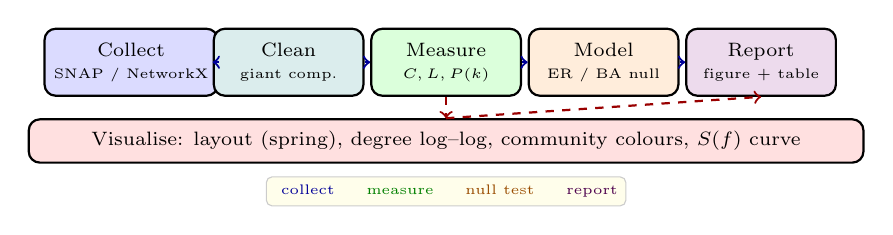
\begin{tikzpicture}[scale=0.80,every node/.style={font=\scriptsize},
  stage/.style={draw,thick,rounded corners=4pt,minimum width=1.9cm,minimum height=0.85cm,align=center}]
\node[stage,fill=blue!14] (a) at (0,0) {Collect\\\tiny SNAP / NetworkX};
\node[stage,fill=teal!14] (b) at (2.5,0) {Clean\\\tiny giant comp.};
\node[stage,fill=green!14] (c) at (5.0,0) {Measure\\\tiny $C,L,P(k)$};
\node[stage,fill=orange!14] (d) at (7.5,0) {Model\\\tiny ER / BA null};
\node[stage,fill=violet!14] (e) at (10.0,0) {Report\\\tiny figure + table};
\foreach \p/\q in {a/b,b/c,c/d,d/e} \draw[->,thick,blue!60!black] (\p)--(\q);
\node[stage,fill=red!12,minimum width=10.6cm,minimum height=0.55cm] (f) at (5.0,-1.25) {Visualise: layout (spring), degree log--log, community colours, $S(f)$ curve};
\draw[->,thick,red!60!black,dashed] (c.south)--(f.north); \draw[->,thick,red!60!black,dashed] (f.north)--(e.south);
\node[font=\tiny,draw=gray!40,fill=yellow!8,rounded corners=2pt,inner sep=3pt] at (5.0,-2.05) {\textcolor{blue!60!black}{$\blacksquare$ collect} \quad \textcolor{green!50!black}{$\blacksquare$ measure} \quad \textcolor{orange!60!black}{$\blacksquare$ null test} \quad \textcolor{violet!60!black}{$\blacksquare$ report}};
\end{tikzpicture}
\caption{Capstone pipeline: from raw data to report. Each stage maps to a chapter: measure (Ch.~1--2), null model (Ch.~4--5), spreading/robustness (Ch.~6--7), applications (this chapter). Visualisation threads through all.}
\label{fig:capstone-pipeline}
\end{figure}

\begin{lstlisting}[language=Python, caption={End-to-end mini-project on Les Mis\'erables co-appearance network.}, label={lst:lesmis}]
import networkx as nx

G = nx.les_miserables_graph()
print(f"LesMis: n={G.number_of_nodes()} m={G.number_of_edges()}"
      f" <k>={2*G.number_of_edges()/G.number_of_nodes():.1f}")
print(f"C={nx.average_clustering(G):.3f}"
      f" L={nx.average_shortest_path_length(G):.2f}")
# Degree heavy tail?
import numpy as np
degs = np.array([d for _,d in G.degree()])
print("max k:", degs.max(), "P(k>10):", (degs>10).mean())
# Communities (Louvain) and central figure
import community as community_louvain
part = community_louvain.best_partition(G)
print("communities:", len(set(part.values())),
      "Q=", round(community_louvain.modularity(part,G),3))
bet = nx.betweenness_centrality(G)
hub = max(bet, key=bet.get)
print("top betweenness:", hub, G.nodes[hub], round(bet[hub],3))
\end{lstlisting}

\begin{lstlisting}[language=Python, caption={Cross-domain comparison: karate (social) vs power grid (tech).}, label={lst:cross-domain}]
import networkx as nx

# Karate (social: assortative, high C) vs synthetic grid-like
karate = nx.karate_club_graph()
# Approximate grid trait: WS lattice-like
grid_like = nx.watts_strogatz_graph(100, 4, 0.02, seed=1)

for name, G in [("karate", karate), ("WS-grid", grid_like)]:
    print(f"\n{name}: n={G.number_of_nodes()} m={G.number_of_edges()}"
          f" C={nx.average_clustering(G):.3f}"
          f" assort={nx.degree_assortativity_coefficient(G):.2f}")
    # Robustness hint: spectral radius (threshold proxy)
    import numpy as np
    rho = max(np.linalg.eigvals(nx.to_numpy_array(G)).real)
    print(f"  rho={rho:.1f} -> lambda_c~{1/rho:.3f}")
\end{lstlisting}

\begin{remark}[Ethics and privacy]\label{rem:ethics}
Network data are sensitive: de-anonymisation via structure alone can re-identify individuals (Narayanan--Shmatikov). Biological and infrastructure data have dual-use risks. Always anonymise, aggregate, and obtain consent; respect SNAP/Twitter/protein-data licences and report limitations. For infrastructure, coordinate disclosure before publishing vulnerabilities.
\end{remark}

\begin{example}[Karate club as a microcosm]\label{ex:karate}
Zachary's karate club (34 nodes, 78 edges) will be your running testbed. Its two ground-truth factions (``Mr.~Hi'' vs ``John A'') let you evaluate community detection (Ch.~3 NMI/ARI), its hubs let you test centrality (Ch.~2: instructor has degree 17), and its $C=0.588$, $L=2.41$ illustrate small-world (Ch.~4: vs ER $C\approx0.14$, $L\approx2.2$ with same $n,m$). Every capstone dataset can be compared to this baseline for intuition before formal tests. Use it to debug your pipeline before scaling to thousands of nodes.
\end{example}

\begin{remark}[Assortativity matters]\label{rem:assortativity}
Social networks are typically assortative (hubs link to hubs, $r>0$); biological and technological nets are often disassortative ($r<0$) because hubs avoid each other to compartmentalise function or cost. Assortativity shapes robustness: assortative nets retain a core under random removal but fragment differently under targeting.
\end{remark}

% ============================================================
\section{Chapter Notes}
Social-network analysis was founded by Moreno (1934) and Milgram (1967) ``six degrees''; modern treatments: Easley--Kleinberg (2010). PPI lethality--centrality: Jeong et~al.\ (2001); \emph{C.~elegans} connectome: Watts--Strogatz (1998) and Varshney et~al.\ (2011). WWW bow-tie: Broder et~al.\ (2000); Internet AS-graph: Faloutsos et~al.\ (1999); power-grid small-world: Watts (1999). For motifs, see Milo et~al.\ (2002). SNAP (Leskovec) and NetworkX provide the datasets used above; always cite the source.

% ============================================================
\section{Exercises}
\label{sec:ch08-exercises}
\begin{enumerate}[label=E8.\arabic*, leftmargin=*, itemsep=0.8em]
    \item \textbf{LesMis full report.} Run the LesMis snippet, then additionally compute degree distribution $P(k)$, plot log--log, estimate $\gamma$ via MLE, and compare $C$ and $L$ to an ER graph with same $n,m$. Is it small-world? Write a 1-page summary with one figure and one table.
    \item \textbf{PPI hub meaning.} Load a PPI network (e.g.\ BioGRID yeast via NetworkX `powerlaw` example or SNAP). Find the top-5 hubs by degree and by betweenness. Are they the same? Look up one hub protein---is it known to be essential? Discuss lethality--centrality.
    \item \textbf{Bow-tie check.} Build a directed 8-node Web toy with a 3-node SCC, 2 IN nodes, 2 OUT nodes, and 1 tendril. Identify each node's bow-tie region via reachability (BFS forward+reverse). What fraction of pairs are mutually reachable?
    \item \textbf{Bipartite projection.} From the karate bipartite view (members $\times$ events), or authors $\times$ papers (Fig.~\ref{fig:bipartite-bowtie}), project onto the second mode and compare clustering before vs after projection. Why does projection inflate $C$?
    \item \textbf{Capstone dataset paper.} Choose one SNAP dataset not used above (e.g.\ email-EuAll, powerGrid, celegans). Carry the full pipeline of Fig.~\ref{fig:capstone-pipeline}: measure, null test, centrality, community, SIR and robustness sweep. Deliver a 2-page report with 3 figures and a table; state one universal and one domain-specific finding.
\end{enumerate}
% End of Chapter 8
